\section{Pseudo-ausências e Background em Modelagem de Distribuição de Espécies}

\subsection{Introdução}

Nas unidades anteriores foram discutidos os fundamentos ecológicos que determinam a distribuição das espécies, os procedimentos para obtenção e tratamento de registros de ocorrência, a delimitação da área acessível (M) e a seleção das variáveis ambientais que representam o espaço ecológico ocupado pelos organismos. Esses componentes constituem a base conceitual necessária para a construção de modelos de distribuição de espécies (Species Distribution Models -- SDMs). Entretanto, antes da aplicação dos algoritmos de modelagem, é necessário compreender um dos desafios metodológicos mais importantes dessa área: a representação das ausências e do ambiente disponível para a espécie.

A modelagem da distribuição geográfica depende fundamentalmente da relação entre os locais onde uma espécie ocorre e as condições ambientais encontradas nesses locais. Em situações ideais, os pesquisadores disporiam simultaneamente de registros confiáveis de presença e ausência para toda a área de estudo. Nesse cenário, seria possível estimar diretamente a probabilidade de ocorrência da espécie em função das variáveis ambientais. Contudo, na maioria dos estudos ecológicos e biogeográficos, especialmente em regiões megadiversas como a Amazônia, os dados disponíveis correspondem quase exclusivamente a registros de presença provenientes de coleções biológicas, inventários florísticos, observações de campo e plataformas de compartilhamento de dados, como GBIF, SpeciesLink e SiBBr \citep{franklin2010mapping}.

A distinção entre presença e ausência constitui um aspecto central da inferência ecológica. Enquanto um registro de presença fornece evidência direta de que a espécie foi observada em determinado local, a ausência representa a constatação de que a espécie não ocorre naquele ambiente ou que não foi detectada durante o processo de amostragem. Essa diferença aparentemente simples possui profundas implicações metodológicas, pois a ausência observada nem sempre corresponde à ausência real da espécie \citep{guisan2017habitat}.

Em Ecologia, costuma-se distinguir três situações distintas relacionadas à ausência. A primeira corresponde à \textit{ausência verdadeira}, situação em que a espécie realmente não ocorre em determinado local devido à inadequação ambiental, restrições históricas ou barreiras biogeográficas. A segunda corresponde à \textit{ausência observada}, caracterizada pela não detecção da espécie durante o levantamento de campo. Nesse caso, a espécie pode estar presente, mas não ter sido registrada devido a limitações amostrais ou dificuldades de detecção. Por fim, existe a chamada \textit{ausência ecológica}, situação em que as condições ambientais são potencialmente adequadas para a ocorrência da espécie, mas fatores históricos, limitações de dispersão ou interações bióticas impedem sua presença local \citep{soberon2007grinnellian}.

A distinção entre esses diferentes tipos de ausência está diretamente relacionada ao conceito de nicho ecológico discutido na Unidade 01. Segundo a formulação de Hutchinson (1957), uma espécie ocupa apenas uma parcela do conjunto de condições ambientais potencialmente adequadas para sua sobrevivência. Consequentemente, áreas ambientalmente favoráveis podem não apresentar registros de ocorrência devido a restrições associadas à dispersão ou à história biogeográfica da espécie. Essa constatação reforça a necessidade de interpretar cuidadosamente os registros de ausência em estudos de modelagem \citep{peterson2011ecological}.

Em razão dessas limitações, os SDMs modernos frequentemente utilizam estratégias alternativas para representar o ambiente disponível à espécie. Em vez de depender exclusivamente de registros de ausência observada, muitos algoritmos empregam pontos de background ou pseudo-ausências para caracterizar as condições ambientais disponíveis na região analisada. A escolha dessas estratégias influencia diretamente o desempenho dos modelos, a interpretação ecológica dos resultados e a capacidade de transferência espacial ou temporal das projeções \citep{elith2009species}.

Nesta unidade serão apresentados os fundamentos conceituais do background ambiental e das pseudo-ausências, destacando suas bases ecológicas, seus métodos de construção e suas implicações para a modelagem de distribuição de espécies. Esses conceitos constituem a ponte entre a caracterização do ambiente disponível, desenvolvida nas Unidades 03 e 04, e os algoritmos de modelagem que serão explorados nas unidades subsequentes.

\subsection{O Problema das Ausências em Modelagem de Distribuição de Espécies}

A obtenção de registros confiáveis de ausência representa uma das maiores dificuldades metodológicas em Modelagem de Distribuição de Espécies. Diferentemente dos dados de presença, que podem ser documentados por meio da observação direta dos organismos, a ausência exige evidências de que a espécie realmente não ocorre em determinado local. Demonstrar a inexistência de um organismo em uma área é uma tarefa consideravelmente mais complexa do que comprovar sua presença \citep{franklin2010mapping}.

Grande parte dos bancos de dados biológicos utilizados em SDM foi originalmente desenvolvida para documentar ocorrências taxonômicas e ampliar o conhecimento sobre a distribuição das espécies. Herbários, coleções zoológicas e bases globais de biodiversidade registram prioritariamente locais onde os organismos foram encontrados. Como consequência, essas bases raramente contêm informações sistemáticas sobre locais onde as espécies foram procuradas e não encontradas \citep{peterson2011ecological}.

Além da limitação dos bancos de dados, existe o problema da detectabilidade. Em Ecologia, a probabilidade de detectar uma espécie durante uma amostragem raramente é igual a um. Mesmo quando a espécie está presente, fatores como densidade populacional reduzida, sazonalidade, comportamento criptográfico, estrutura da vegetação ou limitações metodológicas podem impedir seu registro. Dessa forma, a ausência de observação não implica necessariamente ausência de ocorrência \citep{mackenzie2006occupancy}.

Esse problema é particularmente relevante em florestas tropicais. Espécies arbóreas raras podem ocorrer em baixas densidades e permanecer não detectadas mesmo em inventários extensivos. Em regiões remotas da Amazônia, a baixa intensidade amostral e a dificuldade de acesso ampliam ainda mais a incerteza associada aos registros de ausência. Consequentemente, muitos locais classificados como ausentes podem representar apenas falhas de detecção \citep{guisan2017habitat}.

A incerteza associada às ausências pode produzir dois tipos clássicos de erro em SDM. O primeiro corresponde ao erro de omissão, que ocorre quando áreas adequadas ou ocupadas pela espécie são classificadas incorretamente como inadequadas. O segundo corresponde ao erro de comissão, caracterizado pela classificação de áreas inadequadas como potencialmente adequadas para a ocorrência da espécie. O equilíbrio entre esses dois tipos de erro constitui um dos principais desafios da modelagem ecológica moderna \citep{fielding1997review}.

Do ponto de vista ecológico, a ausência de registros pode resultar de diversos processos distintos. Uma espécie pode estar ausente porque o ambiente é inadequado, porque nunca conseguiu alcançar aquela região, porque foi extinta localmente ou simplesmente porque não foi detectada durante o levantamento. Como esses mecanismos produzem o mesmo resultado observacional — a ausência de registros — torna-se impossível distinguir suas causas apenas a partir dos dados brutos de ocorrência \citep{soberon2007grinnellian}.

Diante desse cenário, pesquisadores passaram a desenvolver abordagens capazes de representar o ambiente disponível sem depender exclusivamente de ausências observadas. Essas estratégias culminaram no desenvolvimento dos conceitos de background ambiental e pseudo-ausências, que atualmente constituem componentes fundamentais dos principais algoritmos de modelagem de distribuição de espécies.

\subsection{Background Ambiental}

O conceito de background ambiental surgiu como uma solução para o problema da ausência de informações confiáveis sobre não ocorrência. Em vez de tentar identificar locais onde a espécie certamente não ocorre, o background busca representar o conjunto de condições ambientais disponíveis para a espécie dentro de uma região geográfica específica \citep{phillips2009sample}.

Sob essa perspectiva, o objetivo não é descrever onde a espécie está ausente, mas caracterizar o universo de condições ambientais que poderiam potencialmente ser utilizadas pelo organismo. Os pontos de background representam amostras do ambiente disponível e funcionam como referência para comparar as condições observadas nos locais de ocorrência. Assim, os modelos passam a responder não apenas onde a espécie ocorre, mas também como as condições ambientais associadas às ocorrências diferem das condições encontradas na paisagem como um todo \citep{elith2011statistical}.

A definição do background possui forte fundamentação ecológica e está diretamente relacionada ao modelo BAM proposto por Soberón (2007). Nesse modelo, a distribuição geográfica observada resulta da interação entre três componentes principais: as condições abióticas adequadas (A), as interações bióticas favoráveis (B) e a área acessível à espécie ao longo de sua história evolutiva e biogeográfica (M). O background deve representar precisamente esse componente M, pois é dentro da área acessível que a espécie teve oportunidade de interagir com os ambientes disponíveis.

A relação entre background e área M é uma das questões mais importantes em SDM. Caso o background seja amostrado em uma região excessivamente ampla, incluindo áreas que jamais estiveram acessíveis à espécie, o modelo poderá interpretar incorretamente ambientes não explorados como ambientes evitados. Esse problema introduz vieses ecológicos e compromete a interpretação dos resultados. Por essa razão, recomenda-se que a construção do background seja sempre restrita à hipótese biogeográfica representada pela área M definida na Unidade 03 \citep{barve2011crucial}.

Do ponto de vista estatístico, o background funciona como uma aproximação da disponibilidade ambiental. Em algoritmos como Maxent, por exemplo, os registros de ocorrência são comparados com milhares de pontos de background distribuídos ao longo da área acessível. O modelo busca identificar quais combinações ambientais diferenciam os locais ocupados dos ambientes disponíveis, estimando assim a adequabilidade ambiental relativa da espécie \citep{phillips2006maximum}.

A interpretação ecológica do background pode ser compreendida por meio de uma analogia simples. Imagine que uma espécie arbórea ocorre em determinados setores da Amazônia. Os registros de presença informam quais condições ambientais estão associadas aos locais ocupados. O background, por sua vez, representa todas as condições ambientais que estavam potencialmente disponíveis dentro da área acessível. A comparação entre esses dois conjuntos permite identificar quais ambientes são selecionados, tolerados ou evitados pela espécie.

Essa perspectiva estabelece uma conexão direta entre as Unidades 03, 04 e 05. A Unidade 03 definiu a área acessível (M), enquanto a Unidade 04 caracterizou o espaço ambiental disponível por meio da seleção das variáveis ambientais. Nesta unidade, esses dois componentes são integrados para construir o background ambiental, que servirá como base para a geração de pseudo-ausências e para a calibração dos modelos de distribuição apresentados nas próximas unidades.

\begin{figure}[H]
	\centering
	\includegraphics[width=0.90\textwidth]{figuras/unidade05/unidade05_background_conceitual.png}
	\caption{Representação conceitual do background ambiental em Modelagem de Distribuição de Espécies. Os registros de ocorrência são comparados com amostras do ambiente disponível dentro da área acessível (M), permitindo caracterizar as condições ambientais utilizadas pela espécie em relação às condições existentes na paisagem.}
	\label{fig:background_conceitual}
\end{figure}

\subsection{Presença--Ausência versus Presença--Background}

Após compreender o conceito de background ambiental, torna-se necessário distinguir duas grandes categorias de modelos amplamente utilizadas em Modelagem de Distribuição de Espécies: os modelos baseados em presença--ausência e os modelos baseados em presença--background. Embora ambos tenham como objetivo estimar a adequabilidade ambiental ou a distribuição potencial das espécies, eles diferem substancialmente na forma como utilizam as informações disponíveis durante a calibração do modelo.

Os modelos de presença--ausência foram originalmente desenvolvidos a partir da tradição estatística clássica, na qual a variável resposta é representada por dois estados mutuamente exclusivos: ocorrência e não ocorrência. Nessa abordagem, cada local amostrado recebe um valor binário, sendo atribuído o valor 1 para presenças e o valor 0 para ausências. A relação entre esses registros e as variáveis ambientais é então utilizada para estimar a probabilidade de ocorrência da espécie ao longo da paisagem \citep{guisan2005predicting}.

Diversos algoritmos amplamente empregados em SDM pertencem a essa categoria. Entre eles destacam-se os Modelos Lineares Generalizados (GLM), os Modelos Aditivos Generalizados (GAM), Random Forest (RF) e Boosted Regression Trees (BRT). Em todos esses métodos, a existência de informações representando locais ocupados e não ocupados é fundamental para que o algoritmo consiga distinguir condições favoráveis de condições desfavoráveis à espécie \citep{elith2009species}.

Entretanto, conforme discutido anteriormente, registros confiáveis de ausência raramente estão disponíveis em bancos de dados biológicos. Como consequência, tornou-se prática comum substituir ausências verdadeiras por pseudo-ausências, que representam locais assumidos como não ocupados para fins de calibração estatística. Assim, a maioria dos SDMs modernos baseados em presença--ausência opera, na realidade, utilizando conjuntos de presença e pseudo-ausência \citep{barbet2012selecting}.

Uma abordagem alternativa foi proposta para lidar com a escassez de dados de ausência. Em vez de comparar locais ocupados com locais presumidamente não ocupados, os modelos de presença--background comparam registros de ocorrência com amostras representativas do ambiente disponível. Nesse caso, o objetivo não é identificar ausências, mas determinar quais características ambientais diferenciam os locais ocupados do conjunto de ambientes existentes na área acessível \citep{phillips2009sample}.

O exemplo mais conhecido dessa abordagem é o algoritmo Maxent (\textit{Maximum Entropy}), que utiliza exclusivamente registros de presença combinados com pontos de background. Durante a calibração, o modelo busca estimar a distribuição de máxima entropia sujeita às restrições impostas pelas condições ambientais observadas nos registros de ocorrência. Dessa forma, o algoritmo identifica quais ambientes apresentam características mais semelhantes às encontradas nos locais ocupados pela espécie \citep{phillips2006maximum}.

Do ponto de vista ecológico, ambas as abordagens procuram responder à mesma pergunta fundamental: quais condições ambientais favorecem a ocorrência da espécie? A diferença está no referencial utilizado para essa comparação. Enquanto os modelos presença--ausência contrastam ambientes ocupados e não ocupados, os modelos presença--background contrastam ambientes ocupados com o conjunto de condições disponíveis na paisagem. Essa distinção é fundamental para interpretar corretamente os resultados produzidos pelos diferentes algoritmos que serão apresentados nas próximas unidades.

\begin{figure}[H]
	\centering
	\includegraphics[width=0.85\textwidth]{figuras/unidade05/unidade05_presenca_ausencia_background.png}
	\caption{Diferenças conceituais entre modelos presença--ausência e modelos presença--background. GLM, GAM, RF e BRT utilizam presenças associadas a ausências ou pseudo-ausências, enquanto Maxent utiliza presenças associadas ao background ambiental disponível na área acessível (M).}
	\label{fig:presenca_ausencia_background}
\end{figure}

\subsection{O que são Pseudo-ausências?}

Pseudo-ausências constituem um dos conceitos mais importantes e, ao mesmo tempo, mais frequentemente mal interpretados em Modelagem de Distribuição de Espécies. O termo refere-se a pontos geográficos selecionados artificialmente para representar condições de não ocorrência da espécie durante o processo de calibração dos modelos. Diferentemente das ausências verdadeiras, as pseudo-ausências não correspondem necessariamente a locais onde a espécie está efetivamente ausente \citep{barbet2012selecting}.

A necessidade de utilizar pseudo-ausências surge diretamente da limitação dos bancos de dados biológicos. Como a maioria das bases de ocorrência registra apenas locais onde a espécie foi observada, torna-se impossível construir modelos binários tradicionais sem algum mecanismo que represente condições de não ocorrência. As pseudo-ausências surgem, portanto, como uma solução prática para permitir a aplicação de algoritmos originalmente desenvolvidos para dados de presença e ausência \citep{franklin2010mapping}.

Do ponto de vista estatístico, as pseudo-ausências funcionam como uma amostra do ambiente disponível que não contém registros conhecidos da espécie. Durante a calibração do modelo, esses pontos recebem o valor 0, enquanto os registros de ocorrência recebem o valor 1. O algoritmo então busca identificar quais combinações ambientais distinguem os dois grupos \citep{elith2009species}.

É importante destacar que pseudo-ausência não significa ausência real. Um ponto selecionado como pseudo-ausência pode, na realidade, ser ambientalmente adequado e até mesmo abrigar populações não amostradas da espécie. Por essa razão, a construção de pseudo-ausências deve ser guiada por hipóteses ecológicas e biogeográficas consistentes, minimizando a probabilidade de selecionar locais efetivamente ocupados \citep{peterson2011ecological}.

\begin{importantbox}
	Pseudo-ausências não representam locais comprovadamente desocupados pela espécie. Elas constituem aproximações estatísticas utilizadas para representar condições de não ocorrência durante a calibração de modelos presença--ausência.
\end{importantbox}

A interpretação ecológica das pseudo-ausências está intimamente associada ao conceito de disponibilidade ambiental. Em termos práticos, esses pontos representam uma amostra dos ambientes aos quais a espécie poderia potencialmente ter sido exposta dentro da área acessível definida pela hipótese M. Consequentemente, a qualidade ecológica da delimitação de M exerce influência direta sobre a qualidade das pseudo-ausências geradas \citep{barve2011crucial}.

Diversos estudos demonstraram que a escolha inadequada das pseudo-ausências pode produzir vieses significativos nas estimativas de adequabilidade ambiental, afetando métricas de avaliação, padrões espaciais de predição e projeções para cenários climáticos futuros. Dessa forma, a geração de pseudo-ausências deixou de ser considerada uma etapa meramente técnica e passou a ser reconhecida como uma das decisões ecológicas mais importantes em SDM \citep{zurell2020standard}.

\subsection{Métodos de Geração de Pseudo-ausências}

A definição de pseudo-ausências constitui uma etapa crítica da modelagem, pois diferentes estratégias de amostragem podem produzir resultados substancialmente distintos. Ao longo das últimas décadas, diversos métodos foram propostos para representar o ambiente disponível e minimizar os efeitos da ausência de dados reais de não ocorrência. Cada abordagem possui vantagens, limitações e pressupostos ecológicos específicos \citep{barbet2012selecting}.

\subsubsection{Pseudo-ausências Aleatórias}

O método mais simples consiste na seleção aleatória de pontos em toda a área de estudo. Nessa abordagem, os locais são amostrados sem considerar a distribuição conhecida da espécie ou a estrutura ambiental da paisagem.

Sua principal vantagem reside na simplicidade operacional e no baixo custo computacional. Entretanto, quando a área de estudo é excessivamente ampla, a estratégia pode incluir ambientes que jamais estiveram acessíveis à espécie, produzindo pseudo-ausências ecologicamente irreais. Isso pode inflar artificialmente o desempenho do modelo e gerar estimativas excessivamente otimistas de adequabilidade ambiental \citep{barve2011crucial}.

\subsubsection{Pseudo-ausências Restritas à Área M}

Uma abordagem ecologicamente mais consistente consiste em restringir a geração de pseudo-ausências à área acessível (M). Nessa estratégia, todos os pontos são amostrados exclusivamente dentro da região que a espécie teve possibilidade histórica de colonizar.

Essa abordagem está diretamente alinhada ao modelo BAM e reduz significativamente a probabilidade de introduzir ambientes inacessíveis ao processo de calibração. Por essa razão, tornou-se uma das estratégias mais recomendadas em estudos contemporâneos de modelagem de distribuição \citep{soberon2007grinnellian,barve2011crucial}.

\subsubsection{Environmental Profiling}

No método conhecido como \textit{Environmental Profiling}, as pseudo-ausências são selecionadas em regiões ambientalmente distintas das condições observadas nos registros de ocorrência. A lógica subjacente é reduzir a probabilidade de incluir locais potencialmente adequados à espécie.

Essa estratégia tende a melhorar a discriminação estatística entre presenças e pseudo-ausências. Entretanto, quando utilizada de forma excessivamente restritiva, pode produzir modelos artificialmente simplificados e com baixa capacidade de generalização \citep{barbet2012selecting}.

\subsubsection{Target Group Background}

O método \textit{Target Group Background} foi desenvolvido para lidar com problemas de viés amostral. Em vez de selecionar pontos aleatórios, utiliza registros de ocorrência de grupos taxonômicos amostrados pelos mesmos observadores, instituições ou programas de inventário.

Essa abordagem procura reproduzir o padrão espacial de esforço amostral presente nos dados originais, reduzindo a influência de vieses geográficos de coleta. Tem sido amplamente utilizada em estudos baseados em grandes bancos de dados de biodiversidade \citep{phillips2009sample}.

\subsubsection{Disk Strategy}

A estratégia conhecida como \textit{Disk Strategy} baseia-se na exclusão de áreas próximas aos registros de ocorrência. Nesse método, pseudo-ausências são geradas apenas além de uma determinada distância mínima em relação às presenças.

O objetivo é reduzir a probabilidade de selecionar locais ocupados, mas ainda não amostrados. A escolha da distância de exclusão deve considerar aspectos biológicos da espécie, como capacidade de dispersão, escala espacial do estudo e resolução dos dados ambientais \citep{vanproosdij2016minimum}.

\begin{table}[H]
	\centering
	\caption{Comparação entre os principais métodos de geração de pseudo-ausências utilizados em Modelagem de Distribuição de Espécies.}
	\label{tab:metodos_pseudoausencias}
	\begin{tabular}{p{3.5cm}p{4cm}p{5cm}}
		\toprule
		\textbf{Método} & \textbf{Vantagens} & \textbf{Limitações} \
		\midrule
		Aleatória & Simples e rápida & Pode incluir áreas inacessíveis \
		Restrita à M & Ecologicamente consistente & Depende de uma boa delimitação de M \
		Environmental Profiling & Reduz sobreposição ambiental & Pode superestimar desempenho \
		Target Group Background & Corrige viés amostral & Requer bases de dados amplas \
		Disk Strategy & Minimiza falsos negativos & Sensível à escolha da distância \
		\bottomrule
	\end{tabular}
\end{table}

Os estudos mais recentes convergem para a ideia de que não existe uma estratégia universalmente superior para todas as situações. A escolha do método deve ser orientada pela biologia da espécie, pela qualidade dos dados disponíveis, pela escala espacial da análise e pela hipótese ecológica que fundamenta o estudo. Em todos os casos, a coerência entre pseudo-ausências, área M e espaço ambiental permanece como um dos princípios fundamentais para a construção de modelos ecologicamente interpretáveis.

\subsection{Quantas Pseudo-ausências Utilizar?}

Após definir a estratégia de geração das pseudo-ausências, surge uma questão inevitável: quantas pseudo-ausências devem ser utilizadas na calibração dos modelos? Embora essa pergunta pareça simples, sua resposta envolve aspectos estatísticos, ecológicos e computacionais que podem influenciar significativamente o desempenho dos modelos de distribuição de espécies.

Nos primeiros estudos de SDM, era comum adotar uma relação equilibrada entre presenças e ausências, utilizando números semelhantes de registros para ambas as classes. Essa prática foi herdada da estatística clássica, onde conjuntos balanceados frequentemente produzem estimativas mais estáveis para modelos binários. Entretanto, o desenvolvimento de algoritmos modernos demonstrou que o número ideal de pseudo-ausências depende do método utilizado, da extensão geográfica da análise e da quantidade de registros de ocorrência disponíveis \citep{pearce2000evaluating}.

Do ponto de vista estatístico, as pseudo-ausências representam uma amostra do ambiente disponível à espécie. Assim como ocorre em processos de amostragem convencionais, amostras muito pequenas tendem a representar inadequadamente a variabilidade ambiental existente na área de estudo. Consequentemente, um número insuficiente de pseudo-ausências pode limitar a capacidade do modelo de distinguir ambientes favoráveis e desfavoráveis, reduzindo seu poder discriminatório \citep{franklin2010mapping}.

Por outro lado, o uso excessivo de pseudo-ausências também pode introduzir problemas. Quando o número de pseudo-ausências é muito superior ao número de presenças, os algoritmos podem se tornar excessivamente influenciados pela classe majoritária, aumentando a probabilidade de superestimar áreas inadequadas e reduzindo a sensibilidade para detectar ambientes potencialmente favoráveis. Esse problema é particularmente relevante em espécies raras ou com distribuição geográfica restrita \citep{barbet2012selecting}.

Um dos trabalhos mais influentes sobre o tema foi realizado por Barbet-Massin et al. (2012), que avaliaram diferentes estratégias de geração e quantidades de pseudo-ausências em diversos algoritmos de modelagem. Os autores demonstraram que o número ótimo de pseudo-ausências varia entre métodos, não existindo uma regra universal aplicável a todas as situações. Os resultados evidenciaram que diferentes algoritmos respondem de maneira distinta ao aumento da quantidade de pseudo-ausências, refletindo diferenças em sua estrutura matemática e em seus mecanismos de aprendizagem.

Para modelos lineares, como os GLMs, frequentemente observa-se bom desempenho quando o número de pseudo-ausências é igual ou moderadamente superior ao número de presenças. Nessas situações, a representação equilibrada das classes tende a produzir estimativas estáveis dos coeficientes e facilita a interpretação ecológica dos resultados \citep{barbet2012selecting}.

Em algoritmos de aprendizagem de máquina, como Random Forest e Boosted Regression Trees, a utilização de conjuntos maiores de pseudo-ausências geralmente melhora a representação da heterogeneidade ambiental disponível. Como esses métodos possuem elevada capacidade de modelar relações complexas e interações entre variáveis, frequentemente se beneficiam de amostras mais extensas do espaço ambiental \citep{elith2008working}.

Na prática, muitos estudos contemporâneos utilizam entre uma e dez pseudo-ausências para cada registro de presença, dependendo da extensão da área de estudo e da resolução espacial dos dados ambientais. Em aplicações continentais ou globais, não é incomum utilizar milhares de pseudo-ausências para representar adequadamente a variabilidade ambiental existente na região analisada \citep{guisan2017habitat}.

Mais importante do que estabelecer um número fixo é garantir que as pseudo-ausências representem adequadamente o ambiente disponível dentro da área M. Uma amostra ecologicamente coerente e espacialmente representativa costuma produzir melhores resultados do que simplesmente aumentar o número de pontos sem considerar sua distribuição ambiental.

\begin{table}[H]
	\centering
	\caption{Recomendações gerais para o número de pseudo-ausências em diferentes algoritmos de Modelagem de Distribuição de Espécies.}
	\label{tab:numero_pseudoausencias}
	\begin{tabular}{p{4cm}p{7cm}}
		\toprule
		\textbf{Algoritmo} & \textbf{Recomendação Geral} \
		\midrule
		GLM & Número semelhante ou moderadamente superior ao de presenças \
		GAM & Relação semelhante à utilizada em GLM \
		Random Forest & Quantidades elevadas podem melhorar a representação ambiental \
		BRT & Beneficia-se de conjuntos amplos de pseudo-ausências \
		Maxent & Utiliza background em vez de pseudo-ausências \
		\bottomrule
	\end{tabular}
\end{table}

\subsection{Influência das Pseudo-ausências nos Modelos}

A escolha das pseudo-ausências influencia diretamente os resultados produzidos pelos modelos de distribuição. Muito além de uma etapa preparatória, a definição desses pontos afeta a estrutura estatística do modelo, as métricas de desempenho, a interpretação ecológica dos resultados e a capacidade de projeção para novas regiões ou cenários climáticos futuros \citep{lobo2010uncertain}.

Uma das primeiras consequências observadas está relacionada às métricas de avaliação. Indicadores amplamente utilizados em SDM, como AUC (Area Under the Curve) e TSS (True Skill Statistic), dependem da comparação entre presenças e ausências ou pseudo-ausências. Alterações na quantidade, localização ou estratégia de geração desses pontos podem modificar significativamente os valores dessas métricas, mesmo quando os registros de ocorrência permanecem inalterados \citep{allouche2006assessing}.

Quando pseudo-ausências são selecionadas em ambientes extremamente distintos daqueles ocupados pela espécie, o problema de classificação torna-se artificialmente simples. Nessas circunstâncias, os modelos tendem a apresentar valores elevados de AUC e TSS, produzindo uma falsa impressão de elevado desempenho preditivo. Esse fenômeno é particularmente comum quando pseudo-ausências são geradas fora da área acessível ou em regiões ambientalmente muito contrastantes \citep{barve2011crucial}.

Outro aspecto importante envolve o sobreajuste (\textit{overfitting}). Quando as pseudo-ausências não representam adequadamente a variabilidade ambiental disponível, os modelos podem aprender padrões excessivamente específicos dos dados de treinamento. Embora isso frequentemente resulte em métricas elevadas durante a calibração, a capacidade de generalização para novas áreas ou períodos climáticos tende a ser reduzida \citep{elith2009species}.

A influência das pseudo-ausências torna-se ainda mais evidente em projeções futuras e reconstruções paleoclimáticas. Modelos calibrados com pseudo-ausências inadequadas podem apresentar extrapolações ambientalmente inconsistentes quando projetados para cenários climáticos distintos. Como consequência, erros introduzidos durante a calibração podem ser amplificados ao longo do processo de transferência espacial ou temporal \citep{peterson2011ecological}.

Do ponto de vista ecológico, pseudo-ausências mal definidas podem alterar a interpretação das relações espécie-ambiente. Variáveis ambientais podem parecer mais ou menos importantes dependendo da distribuição espacial dos pontos utilizados para representar a não ocorrência. Assim, decisões tomadas durante a construção das pseudo-ausências podem influenciar diretamente as conclusões ecológicas derivadas do modelo \citep{franklin2010mapping}.

Essas observações reforçam um princípio fundamental da modelagem ecológica: o desempenho estatístico de um modelo não deve ser interpretado isoladamente. Métricas elevadas somente possuem significado quando associadas a uma construção ecologicamente coerente do conjunto de calibração, incluindo ocorrências, área M, variáveis ambientais e pseudo-ausências.

\subsection{Background no Maxent}

O algoritmo Maxent ocupa uma posição singular entre os métodos de Modelagem de Distribuição de Espécies porque não utiliza pseudo-ausências durante a calibração. Em vez disso, emprega uma abordagem baseada na comparação entre registros de ocorrência e o conjunto de condições ambientais disponíveis na área acessível à espécie, representado pelos pontos de background \citep{phillips2006maximum}.

Essa diferença conceitual frequentemente gera confusão entre iniciantes. Embora tanto pseudo-ausências quanto background sejam utilizados para caracterizar o ambiente disponível, eles possuem significados distintos. As pseudo-ausências são tratadas como registros de não ocorrência durante a calibração de modelos binários. O background, por sua vez, não representa ausência. Ele constitui apenas uma amostra das condições ambientais disponíveis dentro da região analisada \citep{phillips2009sample}.

No Maxent, os registros de ocorrência definem as condições ambientais efetivamente utilizadas pela espécie. Os pontos de background representam todas as condições que estavam potencialmente disponíveis dentro da área acessível. O algoritmo procura então identificar quais características ambientais diferenciam os locais ocupados do conjunto de ambientes existentes na paisagem \citep{elith2011statistical}.

Essa abordagem está diretamente alinhada ao conceito de nicho ecológico desenvolvido por Hutchinson (1957) e ao modelo BAM proposto por Soberón (2007). O background representa a disponibilidade ambiental dentro de M, enquanto as ocorrências representam a parcela efetivamente ocupada pela espécie. O modelo estima, portanto, como a espécie seleciona determinadas condições ambientais dentro do universo de possibilidades disponíveis.

Uma consequência importante dessa abordagem é que os valores produzidos pelo Maxent não devem ser interpretados como probabilidades absolutas de ocorrência. Embora frequentemente apresentados em escalas variando entre 0 e 1, esses valores representam índices relativos de adequabilidade ambiental ou favorabilidade ambiental, dependentes do background utilizado durante a calibração \citep{merow2013practical}.

A definição adequada do background é particularmente importante em Maxent. Quando pontos de background são amostrados em áreas excessivamente amplas, incluindo regiões que jamais estiveram acessíveis à espécie, o algoritmo pode interpretar ambientes não explorados como ambientes inadequados. Esse problema reforça a importância da delimitação da área M discutida na Unidade 03 \citep{barve2011crucial}.

Em aplicações práticas, o Maxent geralmente utiliza milhares de pontos de background distribuídos ao longo da área acessível. Esses pontos fornecem uma representação abrangente da disponibilidade ambiental e permitem que o algoritmo estime padrões complexos de resposta ecológica mesmo quando o número de registros de ocorrência é relativamente reduzido \citep{phillips2006maximum}.

A distinção entre presença--ausência e presença--background constitui uma das diferenças conceituais mais importantes entre os algoritmos de SDM. Enquanto GLM, GAM, RF e BRT dependem da construção explícita de pseudo-ausências, o Maxent utiliza o background ambiental para representar o universo de condições disponíveis à espécie. Compreender essa diferença é essencial para interpretar corretamente os resultados produzidos por cada abordagem e para escolher estratégias de modelagem compatíveis com os objetivos do estudo.

\subsection{Estudo de Caso: Construção de Background e Pseudo-ausências para \textit{Dinizia excelsa}}

Ao longo das unidades anteriores foram estabelecidos os principais componentes necessários para a modelagem da distribuição potencial de \textit{Dinizia excelsa} Ducke, uma das espécies arbóreas emergentes mais emblemáticas da Amazônia. Foram compilados e tratados os registros de ocorrência, delimitada a área acessível (M) e selecionado um conjunto ecologicamente consistente de variáveis ambientais. Nesta seção, esses componentes são integrados para construir o conjunto de calibração que será utilizado pelos algoritmos apresentados nas unidades seguintes.

A construção do background e das pseudo-ausências constitui uma etapa crítica da modelagem porque define o contexto ambiental dentro do qual a distribuição da espécie será interpretada. Conforme discutido anteriormente, o significado ecológico dos resultados depende diretamente da coerência entre os registros de ocorrência, a hipótese biogeográfica representada pela área M e a representação do ambiente disponível \citep{barve2011crucial}.

\subsubsection{Registros de ocorrência utilizados}

Os registros utilizados nesta etapa correspondem ao conjunto de ocorrências de \textit{Dinizia excelsa} previamente submetido aos procedimentos de limpeza, validação taxonômica, correção geográfica e rarefação espacial descritos na Unidade 02. Esses procedimentos tiveram como objetivo reduzir erros associados à georreferência, duplicidade de registros e viés espacial de amostragem, produzindo uma base de dados mais adequada para inferências ecológicas \citep{zizka2019coordinatecleaner}.

Após as etapas de controle de qualidade, o conjunto final de ocorrências passou a representar de forma mais consistente a distribuição conhecida da espécie na Amazônia, servindo como base para todas as análises subsequentes do livro.

\subsubsection{Área acessível (M)}

A geração do background e das pseudo-ausências foi restrita à área acessível (M) definida na Unidade 03. Essa delimitação foi construída considerando a distribuição conhecida da espécie, os limites do bioma Amazônia, barreiras biogeográficas relevantes e informações disponíveis sobre sua ecologia e capacidade histórica de dispersão.

A adoção da área M segue as recomendações propostas por Soberón (2007) e Barve et al. (2011), segundo as quais o ambiente disponível deve ser representado exclusivamente dentro da região que a espécie teve oportunidade de acessar ao longo de sua história evolutiva. Dessa forma, evita-se incluir condições ambientais que jamais estiveram disponíveis à espécie, reduzindo vieses ecológicos durante a calibração dos modelos.

\subsubsection{Construção do background ambiental}

Uma vez delimitada a área M, foi realizada a amostragem do background ambiental utilizando os pixels disponíveis dentro dessa região. Cada ponto de background representa uma amostra das condições ambientais potencialmente disponíveis para \textit{Dinizia excelsa}.

O conjunto de background foi extraído utilizando as nove variáveis ambientais selecionadas na Unidade 04 após os procedimentos de correlação, análise de componentes principais e avaliação do Fator de Inflação da Variância (VIF). Dessa forma, o background passou a representar simultaneamente a disponibilidade geográfica e a disponibilidade ambiental existente dentro da área acessível.

\begin{figure}[H]
	\centering
	\includegraphics[width=0.92\textwidth]{figuras/unidade05/unidade05_background_dinizia.png}
	\caption{Background ambiental utilizado para \textit{Dinizia excelsa}. Os pontos representam amostras do ambiente disponível dentro da área acessível (M), utilizada para a calibração dos modelos de distribuição.}
	\label{fig:background_dinizia}
\end{figure}

A Figura \ref{fig:background_dinizia} ilustra a distribuição espacial do background ambiental utilizado neste estudo. Observa-se que os pontos cobrem toda a extensão da área acessível, representando adequadamente a heterogeneidade ambiental disponível à espécie.

\subsubsection{Geração das pseudo-ausências}

Considerando as recomendações da literatura recente, optou-se por utilizar uma estratégia de pseudo-ausências restritas à área M. Essa abordagem foi escolhida por apresentar maior coerência ecológica e por minimizar a inclusão de ambientes inacessíveis ao longo da história biogeográfica da espécie \citep{barbet2012selecting}.

As pseudo-ausências foram geradas aleatoriamente dentro da área M, excluindo-se os pixels ocupados pelos registros de ocorrência. O procedimento resultou em um conjunto de pontos representando condições ambientais potencialmente disponíveis, mas sem registros conhecidos da espécie.

\begin{figure}[H]
	\centering
	\includegraphics[width=0.92\textwidth]{figuras/unidade05/unidade05_pseudoausencias_dinizia.png}
	\caption{Pseudo-ausências geradas para \textit{Dinizia excelsa} dentro da área acessível (M). Os pontos representam locais utilizados para caracterizar condições de não ocorrência durante a calibração dos modelos presença--ausência.}
	\label{fig:pseudoausencias_dinizia}
\end{figure}

É importante ressaltar que esses pontos não representam ausências verdadeiras. Eles constituem aproximações estatísticas utilizadas para descrever ambientes potencialmente não ocupados durante o processo de modelagem.

\subsubsection{Representação no espaço ambiental}

A interpretação das pseudo-ausências torna-se mais clara quando os dados são visualizados no espaço ambiental. Em vez de analisar apenas a distribuição geográfica dos pontos, essa abordagem permite examinar como presenças, background e pseudo-ausências se distribuem ao longo dos gradientes ambientais considerados pelo modelo.

\begin{figure}[H]
	\centering
	\includegraphics[width=0.90\textwidth]{figuras/unidade05/unidade05_espaco_ambiental_pseudoausencias.png}
	\caption{Representação das ocorrências, pseudo-ausências e background no espaço ambiental de \textit{Dinizia excelsa}.}
	\label{fig:espaco_ambiental_pseudoausencias}
\end{figure}

A Figura \ref{fig:espaco_ambiental_pseudoausencias} evidencia que os registros de ocorrência ocupam apenas uma parcela do espaço ambiental disponível dentro da área M. Essa observação reforça um dos princípios centrais da teoria do nicho ecológico: a espécie não utiliza todas as combinações ambientais disponíveis na paisagem, mas apenas um subconjunto compatível com seus requisitos ecológicos.

\subsubsection{Conjunto final para calibração}

Ao final desta etapa, foram integrados quatro componentes fundamentais:

\begin{enumerate}
	\item registros de ocorrência validados;
	\item área acessível (M);
	\item nove variáveis ambientais selecionadas;
	\item pseudo-ausências ecologicamente consistentes.
\end{enumerate}

Esse conjunto constitui a base de dados que será utilizada para calibrar os modelos GLM, GAM, Random Forest e BRT apresentados nas unidades seguintes. Para o algoritmo Maxent, serão utilizados os registros de ocorrência combinados ao background ambiental definido nesta unidade.

\subsection{Fluxograma de Construção das Pseudo-ausências}

A construção do conjunto de calibração utilizado em SDM envolve uma sequência de etapas ecológicas e estatísticas interdependentes. O fluxograma apresentado na Figura \ref{fig:fluxograma_pseudoausencias} sintetiza o procedimento adotado para \textit{Dinizia excelsa}.

\begin{figure}[H]
	\centering
	\includegraphics[width=0.95\textwidth]{figuras/unidade05/unidade05_fluxograma_pseudoausencias.png}
	\caption{Fluxograma de construção das pseudo-ausências e do background ambiental para Modelagem de Distribuição de Espécies.}
	\label{fig:fluxograma_pseudoausencias}
\end{figure}

O processo inicia com os registros de ocorrência obtidos e tratados na Unidade 02. Em seguida, utiliza-se a hipótese biogeográfica representada pela área M construída na Unidade 03. A partir dessa área são amostrados os pontos de background e geradas as pseudo-ausências, que posteriormente são combinadas às variáveis ambientais selecionadas na Unidade 04. O resultado é um conjunto de dados adequado para a calibração dos algoritmos de modelagem.

\begin{center}
	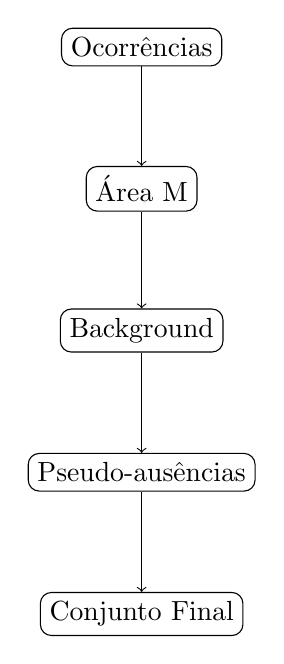
\begin{tikzpicture}[node distance=1.8cm]
		\node (a) [draw, rounded corners] {Ocorrências};
		\node (b) [draw, rounded corners, below of=a] {Área M};
		\node (c) [draw, rounded corners, below of=b] {Background};
		\node (d) [draw, rounded corners, below of=c] {Pseudo-ausências};
		\node (e) [draw, rounded corners, below of=d] {Conjunto Final};
		
		\draw[->] (a)--(b);
		\draw[->] (b)--(c);
		\draw[->] (c)--(d);
		\draw[->] (d)--(e);
	\end{tikzpicture}
\end{center}

\subsection{Boas Práticas para Construção de Pseudo-ausências e Background}

A qualidade ecológica das pseudo-ausências e do background exerce influência direta sobre a confiabilidade dos modelos produzidos. Diversos estudos demonstram que erros nessa etapa podem comprometer todo o processo de modelagem, independentemente da sofisticação do algoritmo utilizado \citep{barbet2012selecting, zurell2020standard}.

A principal recomendação consiste em restringir a geração de pseudo-ausências à área acessível da espécie. A utilização de áreas excessivamente amplas pode introduzir ambientes que jamais estiveram disponíveis ao organismo, produzindo interpretações equivocadas sobre suas preferências ecológicas.

Outro aspecto importante é garantir que o número de pseudo-ausências seja suficiente para representar a heterogeneidade ambiental disponível. Conjuntos muito pequenos tendem a subestimar a variabilidade ambiental, enquanto conjuntos excessivamente grandes podem gerar desequilíbrios estatísticos entre as classes.

Também é recomendável avaliar visualmente a distribuição espacial e ambiental das pseudo-ausências antes da calibração dos modelos. Essa inspeção frequentemente permite identificar problemas relacionados à cobertura geográfica, viés espacial ou superposição excessiva com os registros de ocorrência.

\begin{table}[H]
	\centering
	\caption{Boas práticas para geração de pseudo-ausências e background em Modelagem de Distribuição de Espécies.}
	\label{tab:boas_praticas_pseudoausencias}
	\begin{tabular}{p{4.5cm}p{4.5cm}p{5.5cm}}
		\toprule
		\textbf{Situação} & \textbf{Problema} & \textbf{Recomendação} \
		\midrule
		Pseudo-ausências fora de M & Viés ecológico & Restringir à área acessível \
		Poucas pseudo-ausências & Baixa representatividade & Aumentar a amostragem ambiental \
		Background excessivamente amplo & Ambiente irrealista & Revisar delimitação de M \
		Sobreposição com ocorrências & Ambiguidade ecológica & Excluir áreas ocupadas \
		Viés espacial acentuado & Modelos enviesados & Avaliar distribuição espacial dos pontos \
		Ausência de justificativa ecológica & Interpretação comprometida & Fundamentar a estratégia adotada \
		\bottomrule
	\end{tabular}
\end{table}

Essas recomendações serão fundamentais para interpretar adequadamente os resultados obtidos nas próximas unidades, onde os conjuntos construídos nesta etapa serão utilizados para calibrar os modelos GLM, GAM, Random Forest, BRT e Maxent.
